\documentclass[../../main.tex]{subfiles}
\graphicspath{{../../image/}{../../figure/}}
\begin{document}

\section{真非线性系统的总变差界}\label{section:ch13-总变差界}

此处证明估计\eqref{align:ch13-h-tv}与\eqref{align:ch13-h-lip}，始终在 $U_h$ 的振幅关于 $h$ 一致有界的假设下进行。工具是\cref{theorem:ch13-glimm递减}的下述推论：

\begin{theorem}[总变差的局部界]\label{theorem:ch13-tv局部界}
固定 $0\leqslant\tau<t<\infty$ 与 $-\infty<a<b<\infty$。假设 $\kappa$ 乘以 $U_h(\cdot,t)$ 在区间 $[a-\lambda(t-\tau)-6h,\ b+\lambda(t-\tau)+6h]$ 上的总变差充分小。\footnote{如前，$\lambda$ 表示空间步长与时间步长之比。}则
\begin{align}
TV_{[a,b]}U_h(\cdot,t)\leqslant c_1TV_{[a-\lambda(t-\tau)-6h,\ b+\lambda(t-\tau)+6h]}U_h(\cdot,\tau),
\label{align:ch13-tv-local}
\end{align}
其中 $c_1$ 仅依赖于 $F$。进而，若 $x$ 同时是 $U_h(\cdot,\tau)$ 与 $U_h(\cdot,t)$ 的连续点，且 $\kappa$ 乘以 $U_h(\cdot,t)$ 在区间 $[x-\lambda(t-\tau)-6h,\ x+\lambda(t-\tau)+6h]$ 上的总变差充分小，则
\begin{align}
|U_h(x,t)-U_h(x,\tau)|\leqslant c_5TV_{[x-\lambda(t-\tau)-6h,\ x+\lambda(t-\tau)+6h]}U_h(\cdot,\tau),
\label{align:ch13-osc-local}
\end{align}
其中 $c_5$ 仅依赖于 $F$。
\end{theorem}

\begin{proof}
首先确定非负整数 $\sigma$ 与 $s$，使 $t_\sigma\leqslant\tau<t_{\sigma+1}$ 且 $t_s\leqslant t<t_{s+1}$。接着确定整数 $r_1,r_2$，使 $y_{s+1}^{r_1}<a\leqslant y_{s+1}^{r_1+3}$ 且 $y_{s+1}^{r_2-3}\leqslant b<y_{s+1}^{r_2-1}$。然后令 $r_3=r_1-(s-\sigma)$，$r_4=r_2+(s-\sigma)$。

现按\cref{figure:ch13-锯齿网格曲线}所示构造两条网格曲线 $I$ 与 $J$，步骤如下：$I$ 从采样点 $(y_\sigma^{r_3},t_\sigma)$ 出发，在 $t_\sigma$ 与 $t_{\sigma+1}$ 之间往返锯齿行进，直到到达采样点 $(y_\sigma^{r_3},t_\sigma)$ 处终止。$J$ 从 $(y_\sigma^{r_3},t_\sigma)$ 出发，向``东北''走 $s-\sigma$ 步，到达采样点 $(y_s^{r_1},t_s)$，然后在 $t_s$ 与 $t_{s+1}$ 之间往返锯齿行进，直到到达采样点 $(y_s^{r_2},t_s)$，最后向``东南''走 $s-\sigma$ 步，在 $(y_\sigma^{r_4},t_\sigma)$ 处终止。

\begin{figure}[ht]
\centering
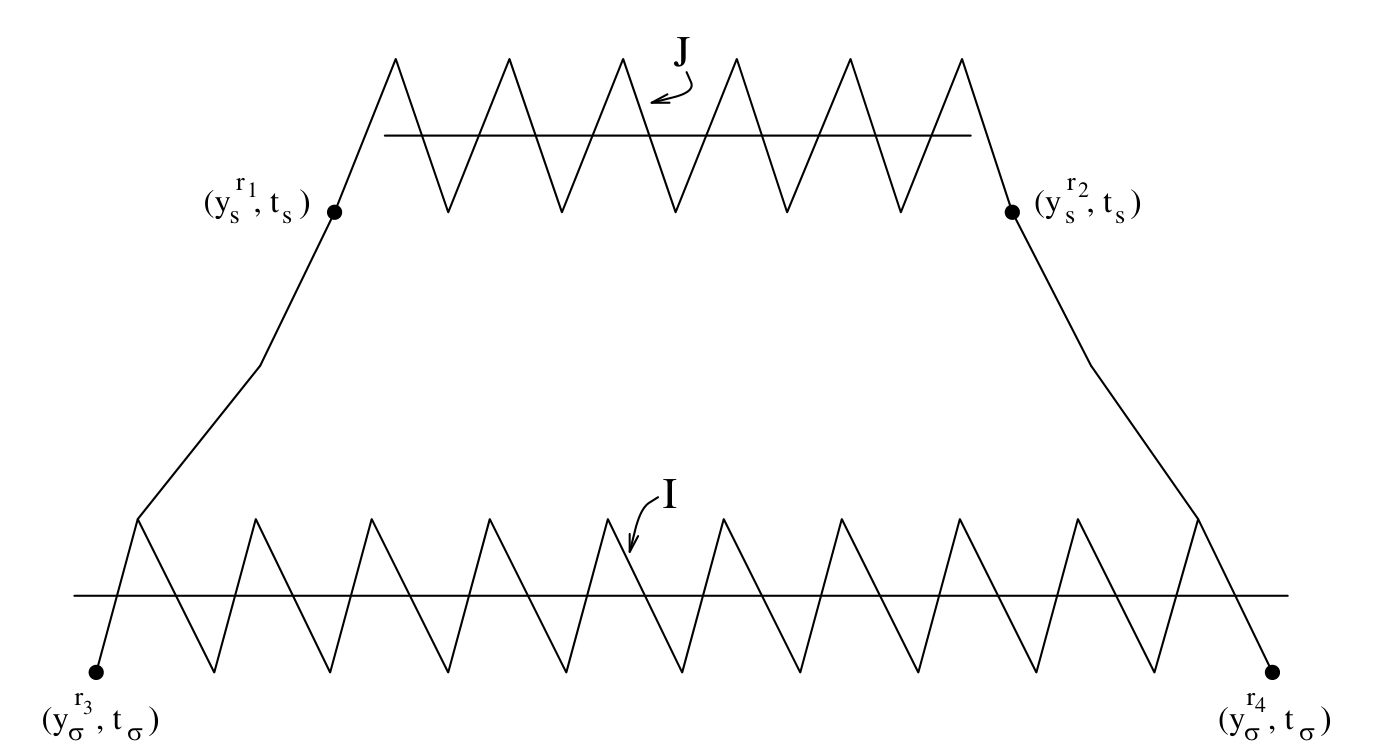
\includegraphics[width=0.9\textwidth]{ch13-fig05-01.png}
\caption{网格曲线 $I$ 与 $J$ 的构造}\label{figure:ch13-锯齿网格曲线}
\end{figure}

显然，
\begin{align}
TV_{[a,b]}U_h(\cdot,t)\leqslant c_6\mathscr{L}(J).
\label{align:ch13-tv-J}
\end{align}
易见 $y_\sigma^{r_3}\geqslant a-\lambda(t-\tau)-6h$，$y_\sigma^{r_4}\leqslant b+\lambda(t-\tau)+6h$。因此，
\begin{align}
\mathscr{L}(I)\leqslant c_7TV_{[a-\lambda(t-\tau)-6h,\ b+\lambda(t-\tau)+6h]}U_h(\cdot,\tau).
\label{align:ch13-L-I}
\end{align}
又 $J$ 是 $I$ 的后继，故若 $2\kappa\mathscr{L}(I)\leqslant1$，\cref{theorem:ch13-glimm递减}蕴含 $\mathscr{L}(J)\leqslant2\mathscr{L}(I)$。把此与\eqref{align:ch13-tv-J}、\eqref{align:ch13-L-I}结合，即得\eqref{align:ch13-tv-local}，其中 $c_1=2c_6c_7$。

给定 $x$，取 $a=b=x$ 重复上述 $I,J$ 的构造。可在 $I$ 上确定一点 $(y',\tau')$ 使 $U_h(y',\tau')=U_h(x,\tau)$，并在 $J$ 上确定一点 $(x',t')$ 使 $U_h(x',t')=U_h(x,t)$。因而
\begin{align}
|U_h(x,t)-U_h(x,\tau)|\leqslant c_8[\mathscr{L}(I)+\mathscr{L}(J)]\leqslant3c_8\mathscr{L}(I).
\label{align:ch13-osc-I}
\end{align}
由\eqref{align:ch13-osc-I}与取 $a=b=x$ 的\eqref{align:ch13-L-I}，推出\eqref{align:ch13-osc-local}，其中 $c_5=3c_7c_8$。证毕。
\end{proof}

对 $\tau=0$、$a\to-\infty$、$b\to\infty$ 应用\eqref{align:ch13-tv-local}，并考虑到 $TV_{(-\infty,\infty)}U_h(\cdot,0)\leqslant TV_{(-\infty,\infty)}U_0(\cdot)$，即验证了\eqref{align:ch13-h-tv}。

最后，把\eqref{align:ch13-osc-local}在 $(-\infty,\infty)$ 上积分，应用 Fubini 定理，并利用\eqref{align:ch13-h-tv}，得到
\begin{align}
\int_{-\infty}^{\infty}|U_h(x,t)-U_h(x,\tau)|\,\mathrm{d}x
&\leqslant c_5\int_{-\infty}^{\infty}TV_{[x-\lambda(t-\tau)-6h,\ x+\lambda(t-\tau)+6h]}U_h(\cdot,\tau)\,\mathrm{d}x\nonumber\\
&=2c_5[\lambda(t-\tau)+6h]\,TV_{(-\infty,\infty)}U_h(\cdot,\tau)\nonumber\\
&\leqslant2c_1c_5[\lambda(t-\tau)+6h]\,TV_{(-\infty,\infty)}U_0(\cdot),
\label{align:ch13-lip-final}
\end{align}
这就建立了\eqref{align:ch13-h-lip}。

\end{document}